% Copyright 2020 by Junwei Wang <i.junwei.wang@gmail.com>
%
% This file may be distributed and/or modified under the
% conditions of the LaTeX Project Public License, either version 1.3c
% of this license or (at your option) any later version.
% The latest version of this license is in
%   http://www.latex-project.org/lppl.txt

% \documentclass[aspectratio=169,compress]{beamer}
\documentclass[aspectratio=169,compress]{beamer}

\usepackage[english]{babel}
\usepackage{metalogo}
\usepackage{listings}
\usepackage{fontspec}
\usepackage{tikz}

% \usetheme{Nord}
\usetheme[style=light]{Nord}


%\usepackage[spanish, es-tabla]{babel}
\usepackage[utf8]{inputenc}
\usepackage{hyperref}




\setmainfont{Yanone Kaffeesatz}
%\setsansfont{Andika New Basic}
\setmonofont{DejaVu Sans Mono}

\setbeamerfont{frametitle}{parent=structure,size=\Large}

\AtBeginSection[]
{
  \begin{frame}[c,noframenumbering,plain]
    \tableofcontents[sectionstyle=show/hide,subsectionstyle=show/show/hide]
  \end{frame}
}

\AtBeginSubsection[]
{
  \begin{frame}[c,noframenumbering,plain]
    \tableofcontents[sectionstyle=show/hide,subsectionstyle=show/shaded/hide]
  \end{frame}
}

\title{Arquitecturas y Organización de Computadoras I}
\subtitle{0: Bienvenida}
\author{Rafael Ignacio Zurita}
\institute{Depto. Ingeniería de Computadoras}
\date{\today}

\begin{document}

\begin{frame}[plain,noframenumbering]
  \maketitle
\end{frame}


\section{Bienvenida}


\begin{frame}[fragile]
  \frametitle{Año 2020 - modalidad virtual}
  Simply include the following code in your preamble:

  \begin{lstlisting}[basicstyle = \ttfamily\small]
\usetheme{Nord}
  \end{lstlisting}

  \bigskip

  By default, the appearance is in dark theme, however you can actively choose a either a light or a
  dark theme.

  \begin{lstlisting}[basicstyle = \ttfamily\small]
\usetheme[style=light]{Nord}
\usetheme[style=dark]{Nord}
  \end{lstlisting}

\end{frame}

\subsection{Colors}

\begin{frame}{Equipo de cátedra y horarios}
  \begin{description}[Snow Storm]
  \item[Docentes]
\begin{small}
    Rafael Ignacio Zurita \texttt{\footnotesize<rafa@fi.uncoma.edu.ar>}\\
\href{mailto:me@example.com}{me@example.com}
    Rodrigo Cañibano \texttt{\footnotesize<rcañibano@fi.uncoma.edu.ar>}\\
    Leandro Insúa \texttt{\footnotesize<leandro.insua@fi.uncoma.edu.ar>}\\
\end{small}
  \item[Horarios]
	Miércoles de 10hs. a 12hs (teoría)\\
	Viernes de 10hs. a 12hs. (práctica)\\
  \item[Exámenes]
	Primer parcial:\\ 
	Segundo parcial:\\
	Recuperatorio integral:
  

  \end{description}
\end{frame}

\subsection{Fonts}

\begin{frame}{Información administrativa}
  \begin{description}[Snow Storm]
  \item[Docentes]
    \textcolor{NordDarkBlack}{NordDarkBlack} \quad \textcolor{NordBlack}{NordBlack}\\
    \textcolor{NordMediumBlack}{NordMediumBlack} \quad \textcolor{NordBrightBlack}{NordBrightBlack}
  \item[Snow Storm]
    \textcolor{NordWhite}{NordWhite} \quad \textcolor{NordBrighterWhite}{NordBrightestWhite}\\
    \textcolor{NordBrightestWhite}{NordBrightestWhite}
  \item[Forest]
    \textcolor{NordCyan}{NordCyan} \quad \textcolor{NordBrightCyan}{NordBrightCyan}\\
    \textcolor{NordBlue}{NordBlue} \quad \textcolor{NordBrightBlue}{NordBrightBlue}
  \item[Aurora]
    \textcolor{NordRed}{NordRed} \quad \textcolor{NordOrange}{NordOrange} \\
    \textcolor{NordYellow}{NordYellow} \quad \textcolor{NordGreen}{NordGreen} \\
    \textcolor{NordMagenta}{NordMagenta}
  \end{description}
\end{frame}



\subsection{Blocks}

\begin{frame}
\begin{block}{Labour Government introduces life saving cancer drug}

    \begin{columns}[onlytextwidth,T]
      \column{\dimexpr\linewidth-30mm-5mm}

      The labour government this week has made available a new treatment
      for a rare form of cancer. The usage of
      Medifix\textsuperscript{\textregistered} in Public hospitals. The
      new drug is expected to save as many as 20 lives per year.

      \column{30mm}
      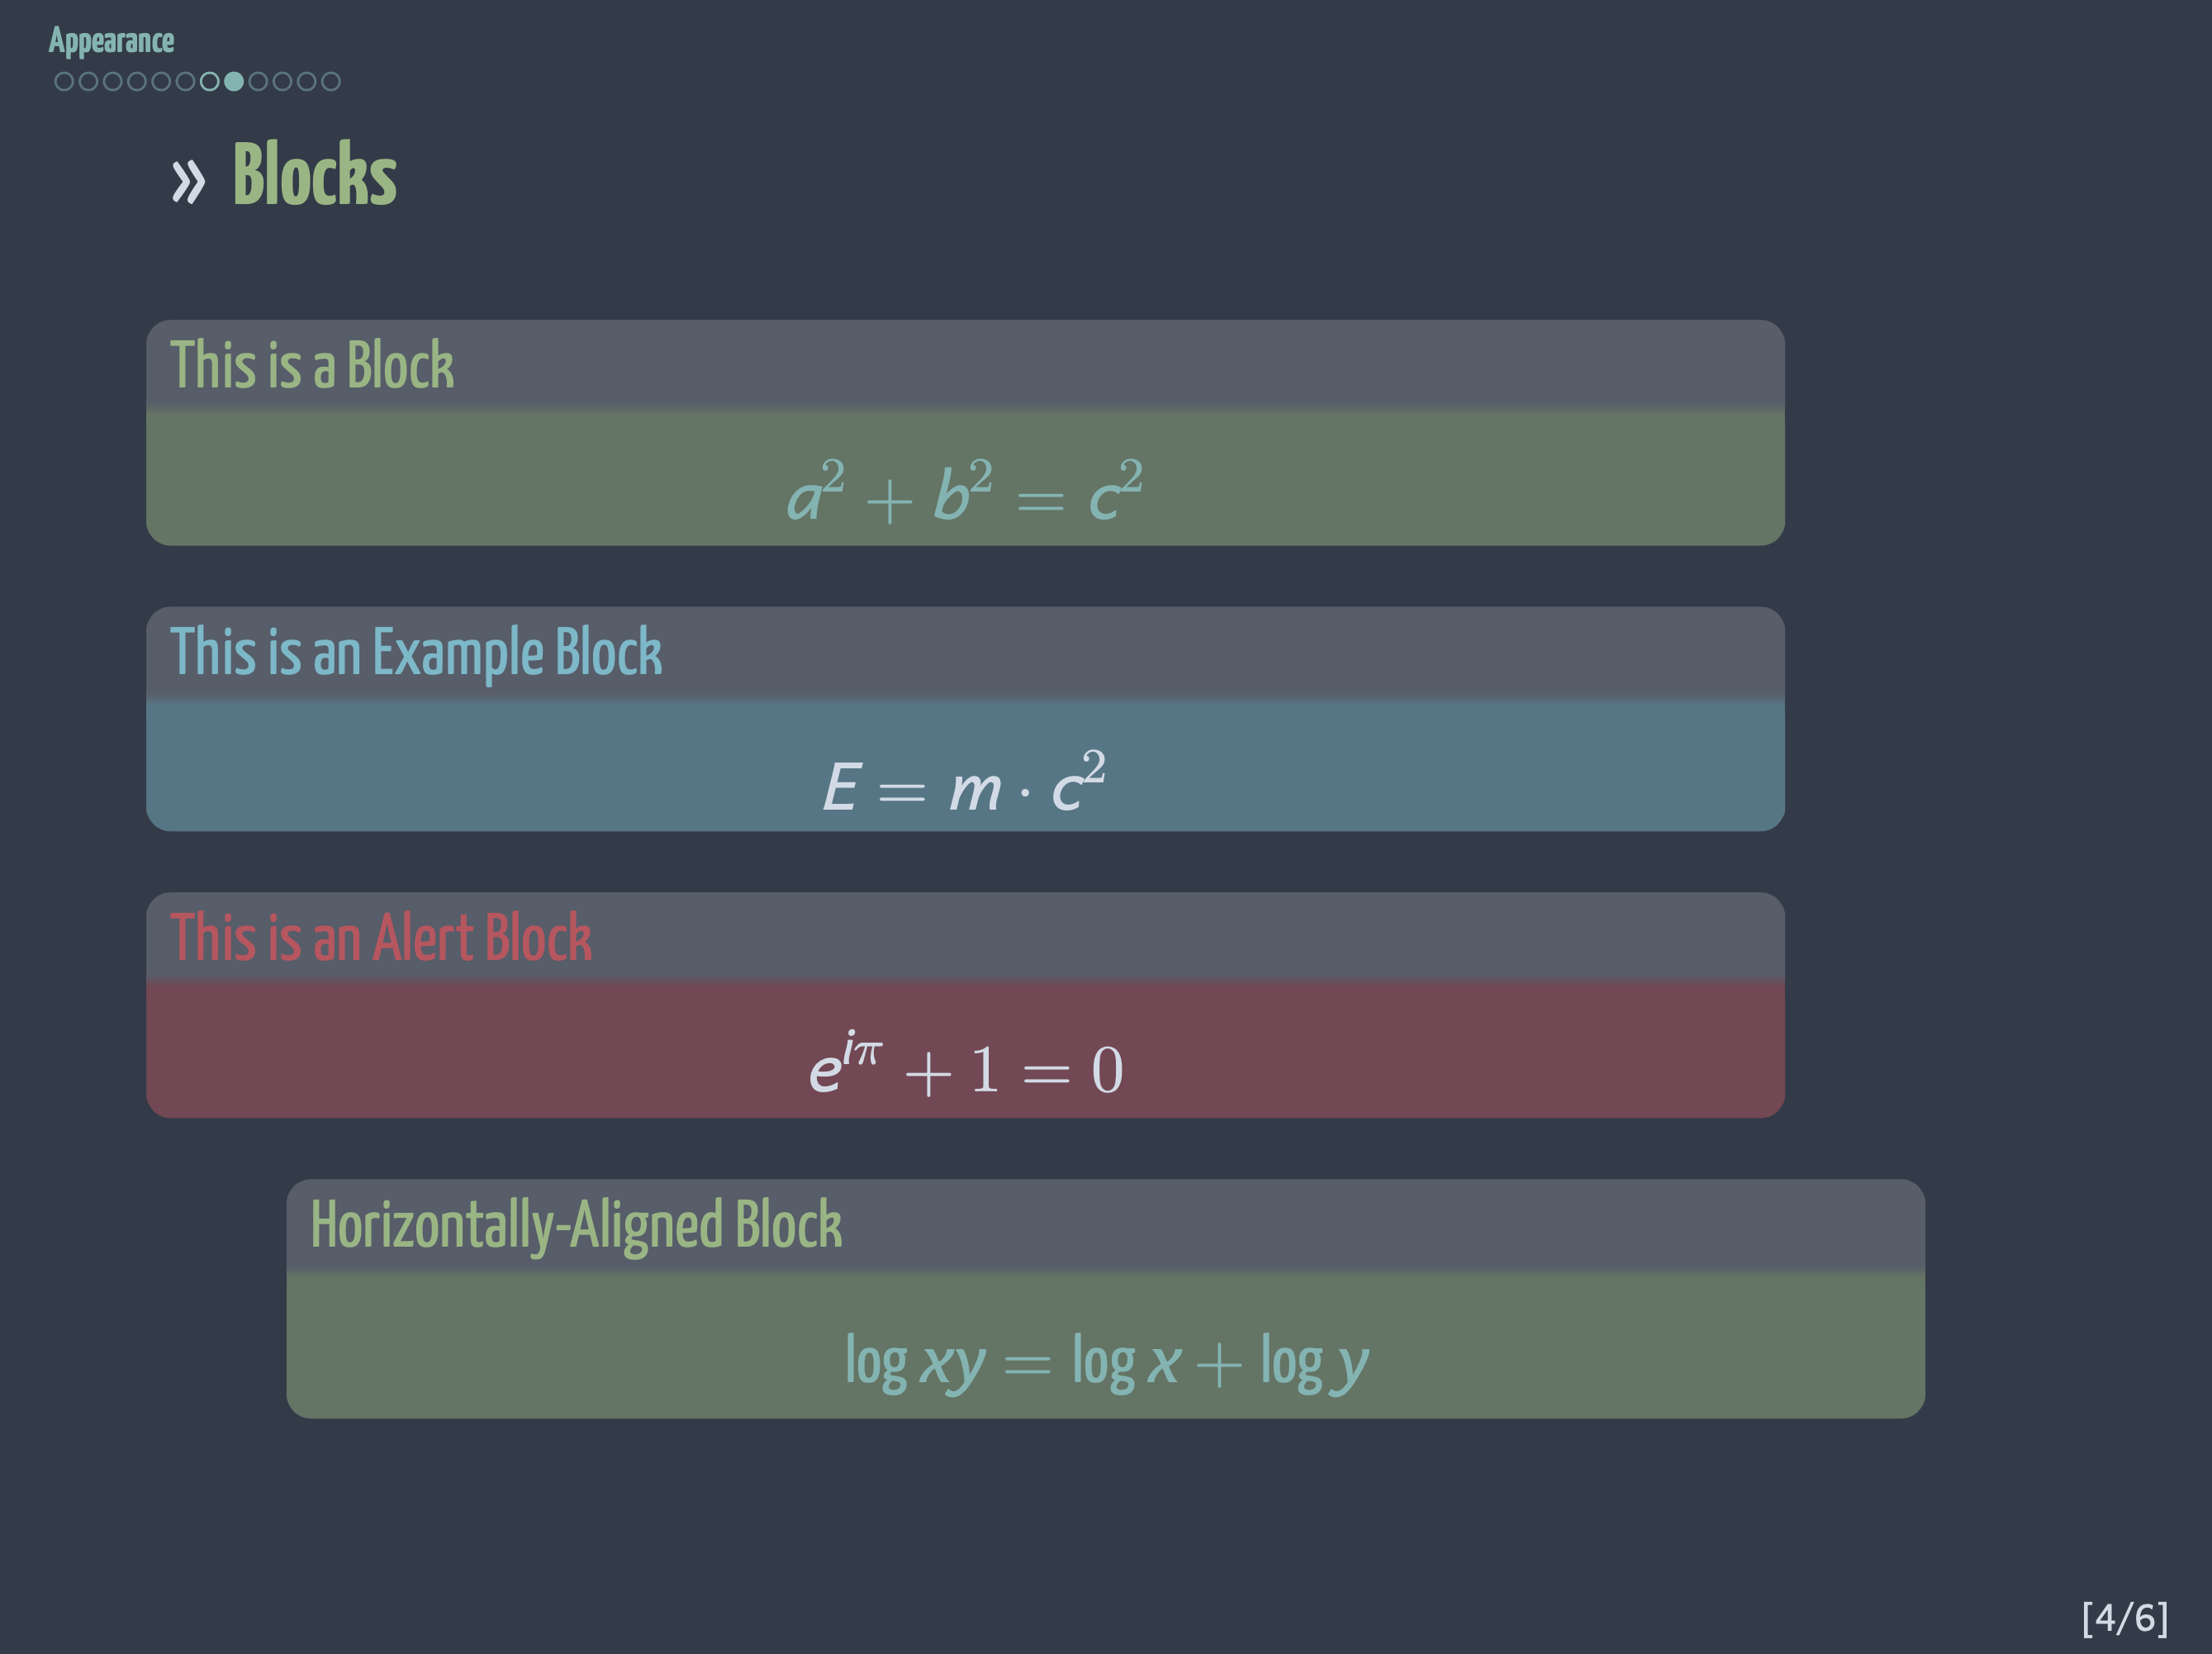
\includegraphics[width=30mm]{dark.png}

    \end{columns}
  \end{block}

\end{frame}



\begin{frame}

    \begin{columns}[onlytextwidth,T]
      \column{\dimexpr\linewidth-60mm-5mm}

      The labour government this week has made available a new treatment
      for a rare form of cancer. The usage of
      Medifix\textsuperscript{\textregistered} in Public hospitals. The
      new drug is expected to save as many as 20 lives per year.

      \column{60mm}
      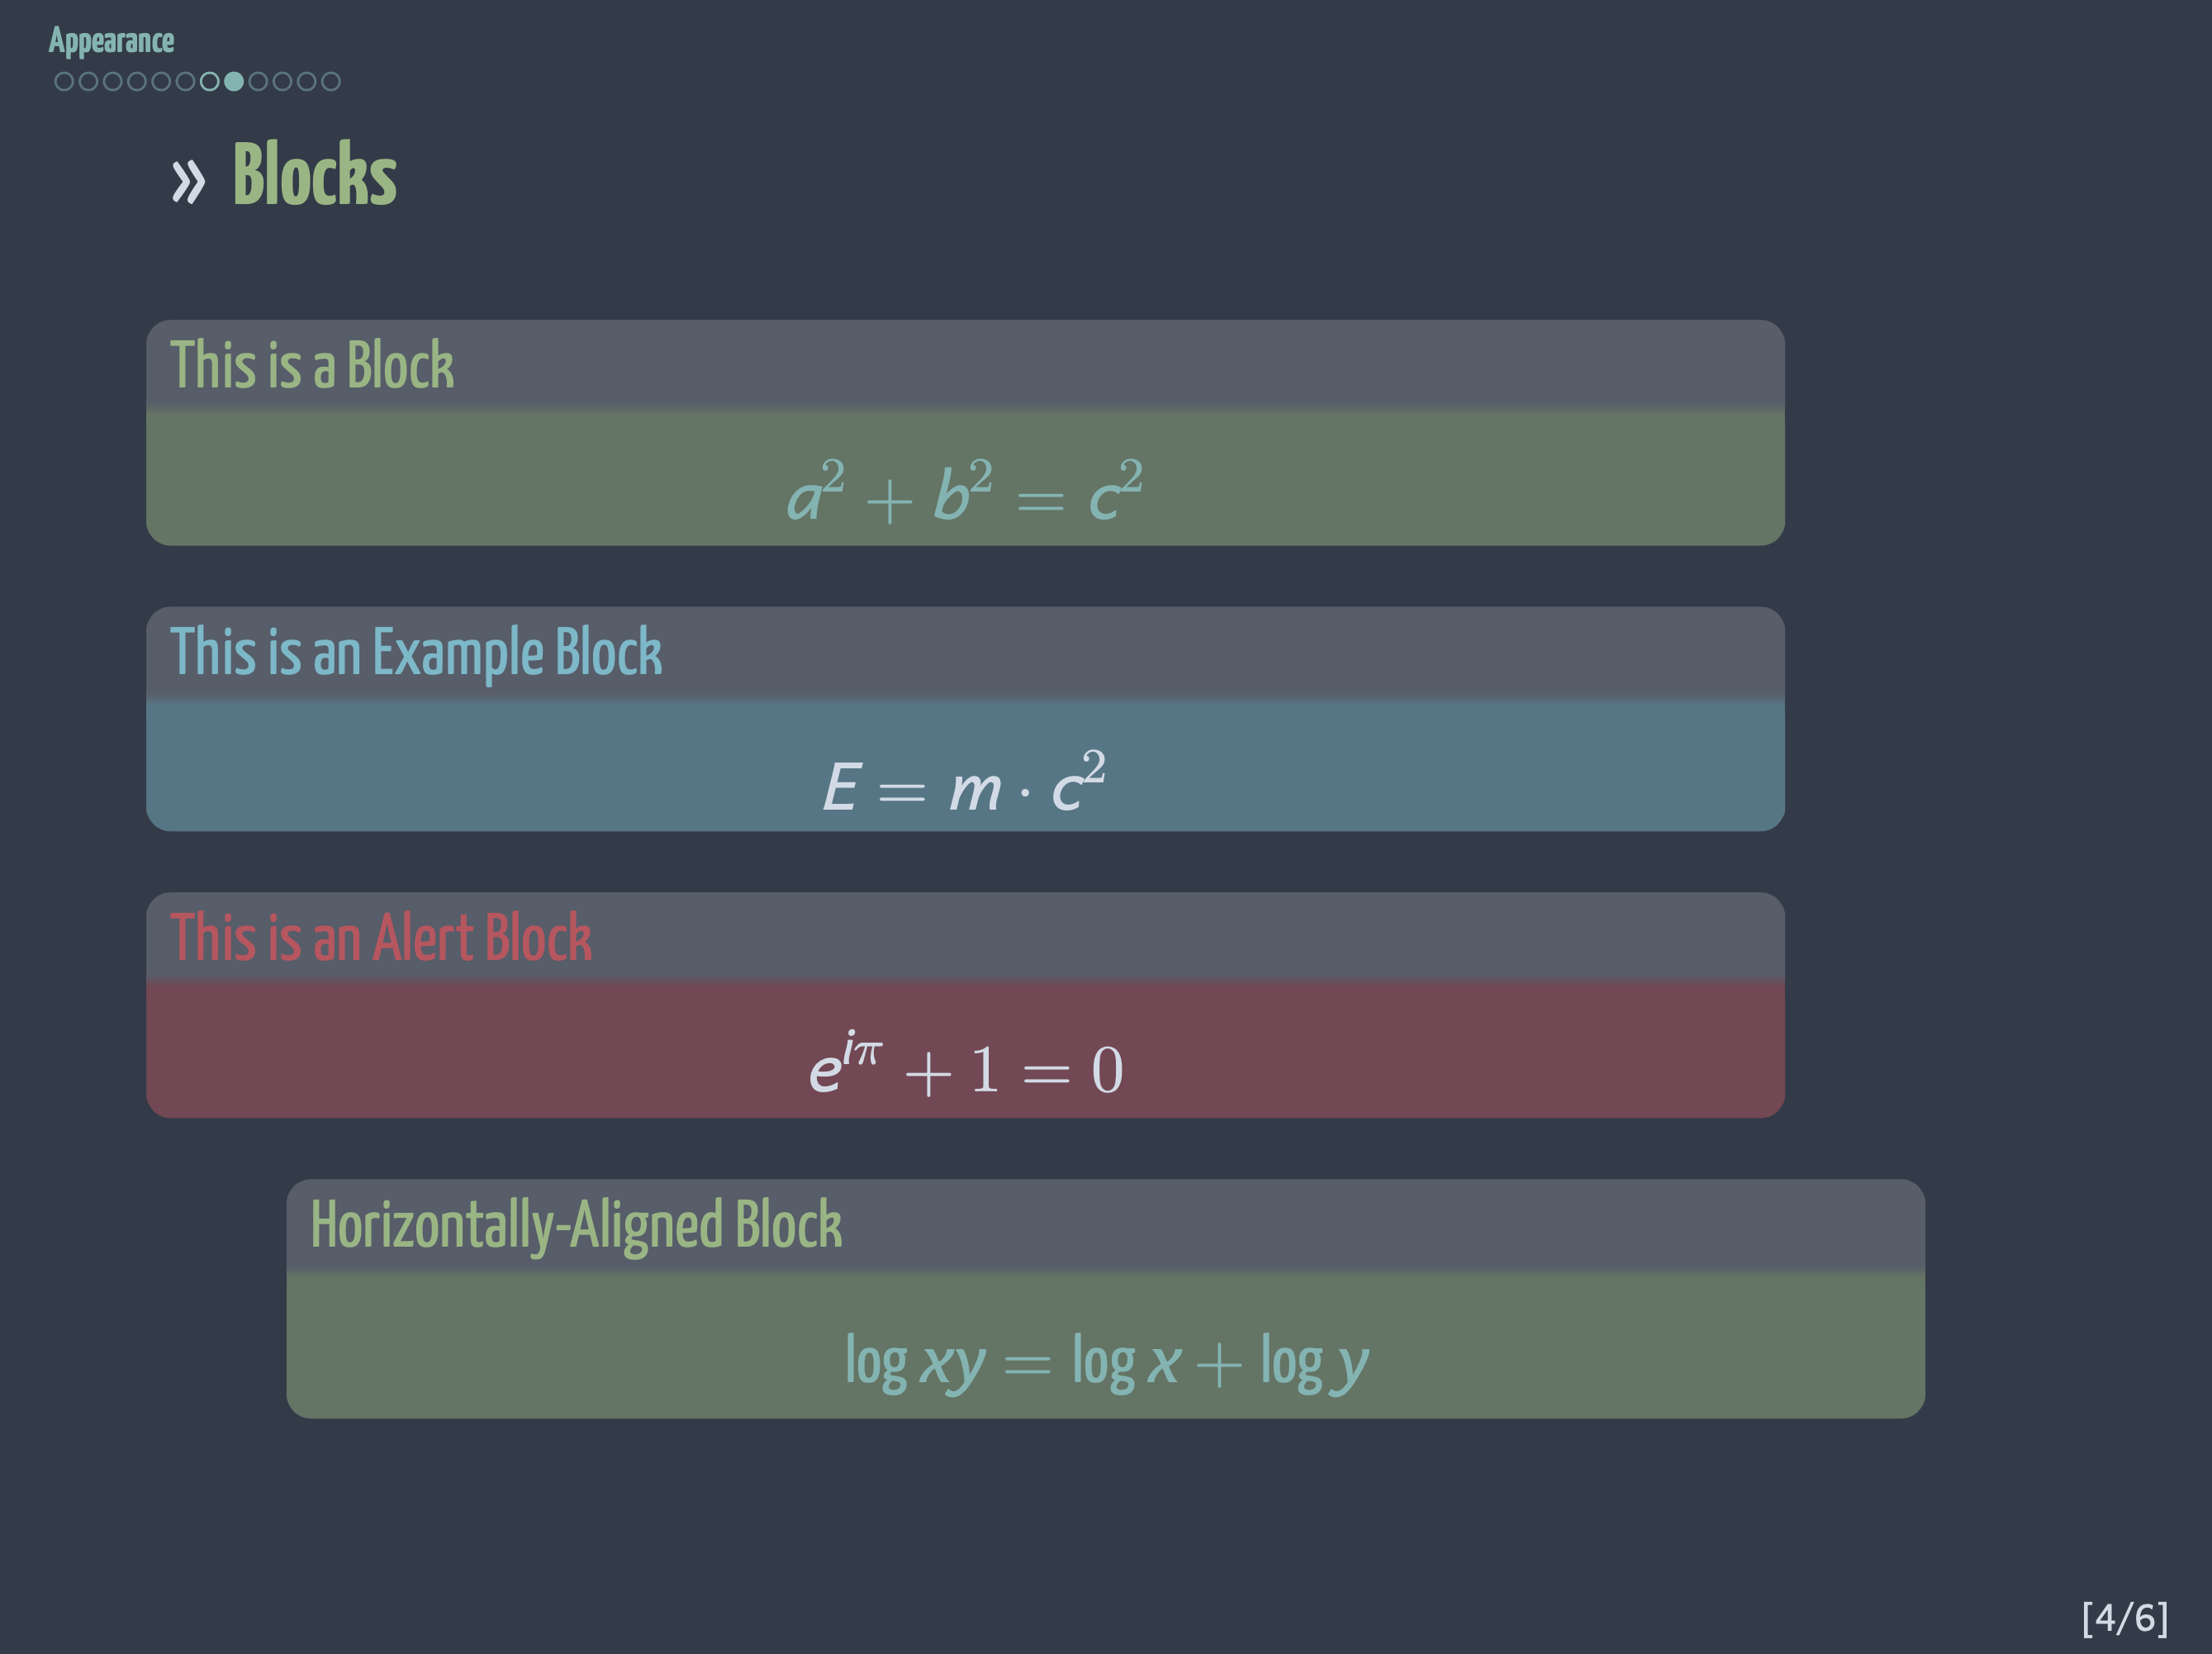
\includegraphics[width=60mm]{dark.png}

    \end{columns}

\end{frame}



\begin{frame}
  \frametitle{Blocks}
  \begin{block}{This is a Block}
    \[
      a^2 + b^2 = c^2
    \]
  \end{block}
  \begin{exampleblock}{This is an Example Block}
    \[
      E = m \cdot c^{2}
    \]
  \end{exampleblock}
  \begin{alertblock}{This is an Alert Block}
    \[
      e^{i\pi} + 1 = 0
    \]
  \end{alertblock}

  \centering
  \begin{minipage}{1.0\linewidth}
    \begin{block}{Horizontally-Aligned Block}
      \[
        \log xy = \log x + \log y
      \]
    \end{block}
  \end{minipage}
\end{frame}

\subsection{Items}

\begin{frame}{Items}
  Itemize
  \begin{itemize}
    \item item 1
    \item item 2
  \end{itemize}

  \bigskip

  Enumerate
  \begin{enumerate}
    \item item 1
    \item item 2
  \end{enumerate}
\end{frame}

\begin{frame}{Motivation and Real-Wordl Applications}
  \begin{itemize}
    \item Why not using secure hardware ?
  \begin{itemize}
    \item not always available 
    \item expensive (to produce, deploy, integrate, update)
    \item usually has a long lifecycle
    \item security breach is hard to mitigate
  \end{itemize}
  \end{itemize}
  \begin{itemize}
    \item Applications
  \begin{itemize}
    \item Digital Content Distribution
    \item Mobile Payment
    \item Digital Contract Signing
    \item Blockchains and cryptocurrencies
  \end{itemize}
  \end{itemize}


\end{frame}



\subsection{Figures}

\begin{frame}{Figures}
  \begin{figure}
    \centering
    \begin{tikzpicture}
      \draw [help lines,NordMagenta,very thick] (0,0) grid (5,4);
    \end{tikzpicture}
    \caption{Credits to Ti\textit{k}Z}
  \end{figure}
\end{frame}

\end{document}

%%% Local Variables:
%%% mode: latex
%%% TeX-master: t
%%% TeX-engine: xetex
%%% End:
